\newcommand{\tensor}[1]{\mathcal{#1}}
\newcommand{\tens}[1]{\tensor{#1}}

\newcommand{\vect}[1]{\textbf{#1}}

\newcommand{\naam}[1]{\textit{#1}}

\newcommand{\R}{\mathbb{R}}
\newcommand{\N}{\mathbb{N}}
\newcommand{\I}{\mathbb{I}}
\newcommand{\ii}{\vect{i}}


\documentclass[master=cws ,masteroption=gs]{kulemt}
\setup{title={Parallellisatie van berekeningen met matrices via OpenCL},
  author={Daan Wendelen},
  promotor={Prof. dr. ir. M. Van Barel},
  assessor={Prof. dr. ir. Ph. Dutr\'e \and Prof. dr. ir. L. De Lathauwer},
  assistant={Dr. ir. L. Sorber}}
% De volgende \setup mag verwijderd worden als geen fiche gewenst is.
\setup{filingcard,
  translatedtitle={Parallelisation of calculations with matrices using OpenCL},
  udc=681.3,
  shortabstract={We kunnen een tensor voorstellen als een meerdimensionale rij. Er zijn algoritmes die de tensor ontbinden in een Canonieke Polyadische Decompositie (CPD). Deze ontbinding kan ook een benadering zijn. In deze masterproef gaan we kernels ontwikkelen om gradi\"ent gebaseerde optimalisatie-algoritmes te ondersteunen. Dit is een groep van algoritmes die op zoek gaan naar de best benaderende CPD voor een gegeven tensor. We definieren ook een doelfunctie. Dit is de Frobeniusnorm van het verschil tussen de tensor die we benaderen en de benadering ervan.
  Na de inleiding beschrijven we de wiskundige concepten die we nodig hebben om de kernels te ontwikkelen. Vervolgens bespreken het programmeermodel van OpenCL en de architectuur van de AMD Radeon HD 6970. Al onze kernels zijn geoptimaliseerd voor deze grafische kaart.
  Nadat we weten hoe OpenCL en de grafische kaart in elkaar zitten gaan we een paar berekeningen doen. Met deze berekeningen onderzoeken we de theoretisch grenzen van de kernels die we gaan ontwikkelen. Nadat de kernels een groen licht gekregen hebben bespreken we stapsgewijs hoe de kernels in elkaar zitten en waarom die zo in elkaar zitten. Bij elke stap doen we ook een paar metingen zodat de effecten van de optimalisaties zichtbaar zijn. We hebben kernels ontwikkeld om de doelfunctie te berekenen en om de gradi\"ent van de doelfunctie te berekenen. We hebben drie kernels ontwikkeld om de doelfunctie te berekenen. Een eerste eenvoudige kernel die heel effici\"ent blijkt te zijn bij grote probleemgroottes. We halen rekenkrachten tot 1610 Gflop/s bij enkele precisie. De twee andere kernels zijn varianten op de eenvoudige kernel die effici\"enter met het geheugen van de grafische kaart om gaan.
We hebben \'e\'en kernel ontwikkeld om de gradi\"ent van de doelfunctie te berekenen, maar die presteert ondermaats.}}
% Verwijder de "%" op de volgende lijn als je de kaft wil afdrukken
%\setup{coverpageonly}
% Verwijder de "%" op de volgende lijn als je enkel de eerste pagina's wil
% afdrukken en de rest bv. via Word aanmaken.
%\setup{frontpagesonly}

% Kies de fonts voor de gewone tekst, bv. Latin Modern
\setup{font=lm}

% Hier kun je dan nog andere pakketten laden of eigen definities voorzien

% Tenslotte wordt hyperref gebruikt voor pdf bestanden.
% Dit mag verwijderd worden voor de af te drukken versie.
\usepackage[pdfusetitle,colorlinks,plainpages=false]{hyperref}
\usepackage[dutch]{babel}
\usepackage{amsfonts, amsmath}
%\usepackage{todonotes}
\usepackage{listings}
%\usepackage{natbib}
\usepackage{graphicx}
\usepackage{pdfpages}
\usepackage{pdflscape}

\lstset{language=C, basicstyle=\footnotesize\ttfamily, keepspaces=true, breaklines=true, tabsize=4,captionpos=t}

\setlength{\parindent}{0pt}
\setlength{\parskip}{1.5ex plus 0.5ex minus 0.5ex}


%\includeonly{hfdst-n}
\begin{document}

\begin{preface}
	Ik wil graag een paar mensen bedanken en ik ga beginnen met mijn promotor Marc Van Barel en mijn begeleider Laurent Sorber. Zonder hun zou deze masterproef er nooit geweest zijn. Ik dank hun voor hun advies en omdat ik altijd bij hun terecht kon met al mijn vragen. Ik wil ook de onderzoeksgroep Numerical Approximation and Linear Algebra Group (NALAG) bedanken voor het ter beschikking stellen van Falcon\footnote{Falcon is een rekenplatform met twee krachtige grafische kaarten en twee krachtige CPU's.}.
	
	Naast mijn promotor en begeleider wil ik ook mijn assessoren Philip Dutr\'e en Lieven De Lathauwer bedanken voor de tijd die ze in mijn masterproef gestoken hebben. Ik wil ook een voormalige assessor, Ares Lagae, bedanken voor de kritische feedback tijdens de tussentijdse presentatie.
	
	Omdat studeren niet gratis is, wil ik graag mijn ouders bedanken voor de financi\"ele ondersteuning van mijn studies.
	Tot slot wil ik ook de rest van mijn familie bedanken voor hun steun.
\end{preface}

\tableofcontents*

\begin{abstract}
	We kunnen een tensor voorstellen als een meerdimensionale rij. Er zijn algoritmes die de tensor ontbinden in een Canonieke Polyadische Decompositie (CPD). Deze ontbinding kan ook een benadering zijn. In deze masterproef gaan we kernels ontwikkelen om gradi\"ent gebaseerde optimalisatie-algoritmes te ondersteunen. Dit is een groep van algoritmes die op zoek gaan naar de best benaderende CPD voor een gegeven tensor. We definieren ook een doelfunctie. Dit is de Frobeniusnorm van het verschil tussen de tensor die we benaderen en de benadering ervan.
  
	Na de inleiding beschrijven we de wiskundige concepten die we nodig hebben om de kernels te ontwikkelen. Vervolgens bespreken het programmeermodel van OpenCL en de architectuur van de AMD Radeon HD 6970. Al onze kernels zijn geoptimaliseerd voor deze grafische kaart.
  
	Nadat we weten hoe OpenCL en de grafische kaart in elkaar zitten gaan we een paar berekeningen doen. Met deze berekeningen onderzoeken we de theoretisch grenzen van de kernels die we gaan ontwikkelen. Nadat de kernels een groen licht gekregen hebben bespreken we stapsgewijs hoe de kernels in elkaar zitten en waarom die zo in elkaar zitten. Bij elke stap doen we ook een paar metingen zodat de effecten van de optimalisaties zichtbaar zijn.
	
	We hebben kernels ontwikkeld om de doelfunctie te berekenen en om de gradi\"ent van de doelfunctie te berekenen.
	We hebben drie kernels ontwikkeld om de doelfunctie te berekenen. Een eerste eenvoudige kernel die heel effici\"ent blijkt te zijn bij grote probleemgroottes. We halen rekenkrachten tot 1610 Gflop/s bij enkele precisie. De twee andere kernels zijn varianten op de eenvoudige kernel die effici\"enter met het geheugen van de grafische kaart om gaan.
	
	We hebben \'e\'en kernel ontwikkeld om de gradi\"ent van de doelfunctie te berekenen, maar die presteert ondermaats.

	
\end{abstract}

% Een lijst van figuren en tabellen is optioneel
%\listoffigures
%\listoftables
% Bij een beperkt aantal figuren en tabellen gebruik je liever het volgende:
\listoffiguresandtables
% De lijst van symbolen is eveneens optioneel.
% Deze lijst moet wel manueel aangemaakt worden, bv. als volgt:
\chapter{Lijst van afkortingen en symbolen}
\section*{Afkortingen}
\begin{flushleft}
	\renewcommand{\arraystretch}{1.1}
  	\begin{tabularx}{\textwidth}{@{}p{12mm}X@{}}
	ADD			& Optel-instructie\\
	b			& bit\\
	B			& Byte\\
    	CPD			& Canonieke Polyadische Decompositie\\
    	CPU			& De gewone processor (Central processing unit)\\
    	CU			& Compute-unit\\
    	double			& Drijvendekommagetal met dubbele precisie\\
    	double2			& Tupel van twee drijvendekommagetallen met dubbele precisie\\
    	double4			& Tupel van vier drijvendekommagetallen met dubbele precisie\\
    	float			& Drijvendkommagetal met enkele precisie\\
    	float2			& Tupel van twee drijvendekommagetallen met enkele precisie\\
    	float4			& Tupel van vier drijvendekommagetallen met enkele precisie\\
    	flop			& Drijvendekomma-operatie\\
    	flop(sp)		& Drijvendekomma-operatie met enkele precisie\\
    	flop(dp)		& Drijvendekomma-operatie met dubbele precisie\\
    	Gi			& $1024^3$\\
    	GPU			& De grafische kaart (Graphics processing unit)\\
    	Ki			& $1024$\\
    	MAD			& Multiply-add ($a = b * c + d$) instructie\\
	MUL			& Vermenigvuldiging-instructie\\
    	Mi			& $1024^2$\\
    	PE			& Processing-element\\
    	SC			& Stream-core\\
  	\end{tabularx}
\end{flushleft}
\newpage

\section*{Symbolen}
\begin{flushleft}
	\renewcommand{\arraystretch}{1.1}
	\begin{tabularx}{\textwidth}{@{}p{12mm}X@{}}
		$\tensor{C}$	& De CPD benadering van $\tensor{T}$.\\
		$f$				& De waarde van $f(\T, \mUUU)$.\\
		$f(\T, \mUUU)$	& De doelfunctie.\\
		$\tens{F}$		& De residu-tensor.\\
		$\mGGG$			& De gradi\"entmatrices.\\
		$I$				& $\forall n = 1, \ldots, N: I_n = I$.\\
		$I_n$			& Het aantal elementen in mode $n$ van \TT.\\
		$N$				& De orde van een tensor.\\
		$R$				& De rang van de CPD.\\
		$t_{ijk}$		& Het ($i$, $j$, $k$)-de element van een tensor $\tens{T}$.\\
		$t_{\ii}$		& Het $\ii$-de element van een tensor $\tens{T}$. Merk op dat $\ii$ een tupel is.\\
		$\tens{T}$		& De tensor die we benaderen.\\
		\UUU{}			& De factormatrices.\\
		\UU{1}			& De factormatrix die we associ\"eren met mode \'e\'en.\\
	\end{tabularx}
\end{flushleft}

% Nu begint de eigenlijke tekst
\mainmatter



\chapter{Inleiding}
\label{inleiding}
Men kan een tensor voorstellen als een $N$-dimensionale rij. Een tensor met twee dimensies noemen we een tweede-orde tensor. Een tweede-orde tensor is niets minder dan een matrix. We kunnen ook tensoren ontbinden.

We kunnen deze tensor ook op de volgende manier ontbinden:

\[
    t_{\ii{}} \approx c_{\ii{}} = \sum_{r=1}^{R} \prod_{n=1}^{N} u^{(n)}_{i_{n}r}
\]
\begin{center}
met $\ii{} \in \I$, $R \in \N_0$, $\mUU{n} \in \R^{I_n \times R}$ \\ en $ \I = \{\ii{} \in \N_0^N | \forall n \in [1, N]: i_n \in [1, I_n]\}$
\end{center}

We noemen deze ontbinding de Canonieke Polyadische Decompositie (CPD). De Canonieke Polyadische Decompositie 

Er bestaan softwarepakketten, waaronder Tensorlab \cite{tensorlab}, die enkele algoritmes implementeren om de CPD te berekenen. De schrijver heeft echter nog geen bewijs gevondezen die er op wijzen dat er al veel onderzoek gedaan is naar het versnellen van deze algoritmes met behulp van OpenCL/CUDA.

\section{Doelstellingen}

Het doel van deze masterproef is om deze algoritmes te ondersteunen met de rekenkracht een grafische kaart. We maken hiervoor gebruik van OpenCL. We gaan op zoek naar rekenintensieve delen uit het algoritme en we gaan die parallelliseren. Maar niet alle algoritmes zijn hiervoor geschikt. Sommige algoritmes zijn gelimiteerd door de bandbreedte. Voor dit soort algoritmes heeft het weinig zin om het uit te voeren op de grafische kaart. Er zijn ook andere algoritmes die men niet kan parallelliseren. Een voorbeeld hiervan is het genereren van recursieve reeksen. Het eerste wat we dus gaan onderzoeken is of het algoritme wel gebruik kan maken van de volledige rekenkracht van de grafische kaart.

Als een deel van het algoritme geschikt is om te parallelliseren, gaan we een zo optimaal mogelijke kernel ontwikkelen. We mikken op een implementatie die minstens \'e\'en Gflop/s kan halen. We berekenen de rekenkracht door het aantal flop's die een optimale implementatie nodig heeft te delen door de tijd die we nodig hebben om dit uit te voeren op de grafische kaart. We gaan ook onderzoeken onder welke omstandigheden de grafische kaart effici\"ent werkt.

De stukken die we parallelliseren zijn op hun eigen niet ze veel waard. Daarom is het ons doel om ze te integreren in \'e\'en van de vele algoritmes die er al bestaan.

\section{Overzicht}
We beginnen met 
\chapter{Tensoren}
\label{h:tensoren}

\todo{intro + vermelden parafrazering + misschien titel CPD noemen}

\section{Tensoren}
Men kan een tensor voorstellen als een $N$-dimensionale rij. We spreken dan over een $N$-de-orde tensor $\tensor{T}$. $\tensor{T}$ heeft $N$ modes en orde is gelijk aan $N$. Formeel schrijven we $\tensor{T} \in \R^{I_1 \times \dotsb \times I_N}$. $I_n$ is gelijk aan het aantal elementen in mode $n$. Tensoren zijn ook gedefini\"eerd voor complexe getallen, maar we gaan ons beperken tot de rationale getallen.


Een element van een derde-orde tensor $\tensor{T}$ noteren we als $t_{ijk}$. $i$ komt overeen met de eerste mode, $j$ met de tweede en $k$ met de derde mode. Een element van een $N$-de-orde tensor schrijven we als $t_\ii$ met $\ii \in \I$. We defini\"eren de indexverzameling $\I$ als de verzameling van alle vectoren die een geldige index van de tensor zijn.
\[
    \I = \{\ii \in \N^N | \forall n \in [1, N]: i_n \in [1, I_n]\}
\]

\todo{Vergelijking met matrix en eventueel vector}
\todo{Is het correct om te zeggen dat een matrix een tweede-orde tensor is? En omgekeerd?}

Tensoren kunnen met elkaar opgeteld worden. $\tens{A} + \tens{B} = \tens{C}$ als en slechts als:
\[
	\forall \ii \in \I: c_\ii = a_\ii + b_\ii
\]

Het is ook mogelijk om de Frobeniusnorm te nemen van een tensor. Deze norm is gelijk som van de kwadraten van alle elementen van de tensor. Wanneer we over de norm van een tensor spreken, spreken we altijd over de Frobeniusnorm.
\[
    ||\tens{T}|| = ||\tens{T}||^2 = \sum_{\ii \in \I} t_\ii^2
\]

\todo{notaties}

\section{Canonieke Polyadische Decompositie (CPD)}
We kunnen een tensor $\tens{T}$ benaderen met de Canonieke Polyadische Decompositie, afgekort CPD.\todo{referentie} Deze ontbinden kunnen we als volgt defini\"eren:
\[
    t_\ii \approx c_\ii = \sum_{r=1}^{R} \prod_{n=1}^{N} u^{(n)}_{i_{n}r} \qquad \text{met $\ii \in \I$}
\]
\todo{Tekening, nog wat uitleg + toepassingen}
\todo{Naam voor 'u' opzoeken of verzinnen. Misschien factormatrix ofzo}
\todo{Dat ding van de rank waarbij een tensor 50proc kans benadering exact is.}
\chapter{Algoritme}
\todo{Eventueel meervoud}
\label{h:algo} 

\begin{align*}
    \tens{F} &= \tens{C} - \tens{T}\\
    \tens{F} &= \left( \sum_{r=1}^{R} \prod_{n=1}^{N} u^{(n)}_{i_{n}r} \right) - \tens{T} \qquad \text{met $\ii \in \I$}
\end{align*}

\begin{align*}
    g^{(n)}_{ir} 	&= \frac{\partial f}{\partial u^{(n)}_{ir}}\\
					&=\frac{\partial}{\partial u^{(n)}_{ir}} \frac{1}{2}\sum_{\ii \in \I}\left(c_\ii - t_\ii \right)^2\\
					&= \frac{1}{2} \sum_{\substack{\ii \in \I\\ \ii_n = i}} \frac{\partial}{\partial u^{(n)}_{ir}} \left(c_\ii - t_\ii \right)^2\\
					&= \frac{1}{2} \sum_{\substack{\ii \in \I\\ \ii_n = i}} 2 \left(c_\ii - t_\ii \right) \frac{\partial c_\ii}{\partial u^{(n)}_{ir}}\\
					&=\sum_{\substack{\ii \in \I\\ \ii_n = i}} f_\ii \frac{\partial}{\partial u^{(n)}_{ir}} \sum_{r'=1}^{R} \prod_{n'=1}^{N} u^{(n')}_{i_{n'}r'}\\
					&=\sum_{\substack{\ii \in \I\\ \ii_n = i}} f_\ii \prod_{\substack{n'=1\\n'\neq n}}^{N} u^{(n')}_{i_{n'}r}\\
\end{align*}
\todo{toepassen op 3D om te verduidelijke / eerst uitwerken voor 3D}
\todo{algemeen alles voor 3D doen}
\chapter{OpenCL}
\label{h:opencl} 
\todo{aangeven voor opencl dat engels gebruikt wordt}
\todo{PE ook gekend als SC}
OpenCL is een framework voor het uitvoeren van parallelle berekeningen. Deze berekeningen kunnen uitgevoerd worden op \'e\'en of meerdere gewone processoren (CPU) of op \'e\'en of meerdere grafische kaarten. Een CPU of een GPU noemen we een apparaat (device).

\section{Het model}
In dit hoofdstuk beschrijven we de voornaamste OpenCL-concepten. Deze zijn onafhankelijk van het apparaat en zelfs van het soort apparaat.
\subsection{Verdeling van het werk}
\todo{Misschien concepten uitleggen adhv het voorbeeld ipv het voorbeeld te gebruiken om de concepten beter uit te leggen}
Een reeks van een instructies die parallel uitgevoerd kan worden noemen we een kernel. De eenheid van werk dat door een kernel verwerkt wordt noemen we een work-item. Het apparaat voert de kernel, in parallel, uit op de work-items. Een work-item komt dus overeen met \'e\'en thread \todo{Van hier tot einde zin miss weglaten}waarbij elke thread dezelfde kernel uitvoert. Het aantal work-items is meestal afhankelijk van de invoer van het algoritme.

Neem als voorbeeld het optellen van twee vectoren. \vect{c} = \vect{a} + \vect{b}. We kunnen dit op een seri\"ele manier berekenen als volgt:
\lstset{language=C, basicstyle=\footnotesize\ttfamily, keepspaces=true}
\begin{lstlisting}
void sum(const double a[], const double b[],
        double c[], int N)
{
    for(int index = 0; index < N; index++)
    {
        c[index] = a[index] + b[index];
    }
}
\end{lstlisting}
We kunnen dit herschrijven naar:
\begin{lstlisting}
void sum(const double a[], const double b[], double c[], int N)
{
    for(int index = 0; index < N; index++)
    {
        inner(a, b, c, index);
    }
}
void inner(const double a[], const double b[], double c[],
    const int index)
{
    c[index] = a[index] + b[index];
}
\end{lstlisting}
In welke volgorde we de index kiezen maakt eigenlijk niets uit. We kunnen deze berekening dus makkelijk in parallel berekenen.
Een OpenCL-kernel uit een programma die dezelfde berekening doet kan er als volgt uitzien:
\begin{lstlisting}
__kernel void innerKernel(__global const double a[],
    __global const double b[], __global double c[])
{
	int i = get_global_id(0);
	c[i] = a[i] + b[i];
}
\end{lstlisting}
Het eerste dat opvalt is dat er een paar keywords zoals \naam{\_\_kernel} en \naam{\_\_global} zijn bij gekomen. \naam{\_\_kernel} geef aan dat de functie een kernel is die gelanceerd kan worden. \naam{\_\_global} geeft aan dat het om globaal geheugen gaat. (Zie \ref{h:opencl:geheugen})

Wat echter veel belangrijker is, is dat de parameter \naam{N} verdwenen is. Waar we vroeger \naam{inner} \naam{N} keren na elkaar uitvoerden, gaan we nu \naam{innerKernel} \naam{N} keer in parallel uitvoeren. Er zijn dus \naam{N} work-items. 

\todo{miss dit erbij zetten, misschien laten vallen}Wanneer we een kernel lanceren, geven we ook mee hoeveel work-items het apparaat moet verwerken.

In dit voorbeeld komt \'e\'en element uit de vector overeen met \'e\'en work-item, maar dit moet niet altijd zo zijn. De kernel gebruikt \naam{get\_global\_id(0)} om te achterhalen welk work-item verwerkt wordt.

\todo{NDRange uitleggen + NDRange -> 1DRange/3DRange}

\todo{Work-group uitleggen}

\subsection{Geheugen}
\label{h:opencl:geheugen}
OpenCL kent drie soorten geheugen:
\begin{itemize}
    \item Privaat geheugen: enkel toegankelijk binnen work-item.
    \item Lokaal geheugen: gedeeld met alle work-items in binnen een work-group, niet toegankelijk buiten de work-group.
    \item Globaal geheugen: toegankelijk voor alle work-items.
\end{itemize}

Gegevens in het RAM-geheugen kunnen enkel gekopi\"eerd worden naar het globaal geheugen. Een work-item kan dan de gegevens lezen uit het globaal geheugen en opslaan in het privaat geheugen. Work-items kunnen ook gegevens schrijven naar het lokaal geheugen. Deze gegevens kunnen dan door andere work-items binnen dezelfde work-group gelezen worden. \todo{tekening: GG, WI, WG, LG, PG}

\subsection{Synchronisatie}

\section{<stuff over cpu en gpu>}


\section{Architectuur AMD Radeon HD 6970}
\subsection{Rekending}
\todo{rename}

Wanneer we een kernel lanceren gaat de GPU de work-groups verdelen over de compute-units. Elke compute-unit (CU) heeft \'e\'en command-processor die verantwoordelijk is voor het selecteren en ophalen van de instructies. Omdat elke CU een eigen command-processor heeft, werken CU's volledig zelfstandig en los van alle andere CU's. \todo{verschil verschillende producten binnen familie is aantal CU's} De compute-unit bestaat, naast de command-processor, ook uit 16 processing-elementen (PE). Alle processing-elementen binnen een compute-unit worden aangestuurd door de command-processor in de compute-unit. Hierdoor voeren alle processing-elementen altijd dezelfde instructie uit.

Zo \'e\'en instructie is 128 bits lang en bestaan eigenlijk uit vier 32-bit instructies. Een 128-bit instructie noemen we een very long instruction word (VILW). Een processing-elementen bestaat uit vier ALU's die elk een 32-bit instructie uitvoeren. Sommige instructies zijn te zwaar om met \'e\'en ALU uit te voeren. Daarom kunnen twee of vier ALU'a samengenomen worden om de zware instructie uit te voeren.\todo{<TODO>}

Misschien een beetje over andere families schrijven om context meer context. Is wel info die niet bijdraagt tot het begrijpen van de ontwerpbeslissingen vd kernels
\todo{</TODO>}

\todo{Wavefront en relatie met work-items (misschien mapping hardware <-> workitems een apart hfdstk}

\todo{Optimalisaties}

\todo{tekening uit slide/handleiding}
\todo{Ultra-Threaded Dispatch Processor}
\todo{latency van 8 cycli}

\subsection{Geheugen}

\subsubsection{Lokaal geheugen}
Elke compute-unit heeft 32KiB lokaal geheugen. Dit geheugen wordt gedeeld door alle work-groups \todo{enkel op dat moment gescheduled zijn} op de compute-unit. Het is voor een work-group echter niet mogelijk om te communiceren met een andere work-group via dit lokaal geheugen. Het lokaal geheugen bestaat uit 32 banken die elk vier bytes breed zijn. Dit betekent dat de eerste 4 bytes in de eerste bank gaan, de volgende vier in de tweede enzovoorts. De 129ste byte gaat terug in de eerste bank. ($4 \times 32 = 128$)

Elk processing-element kan elke cyclus twee vierbyte aanvragen doen. Deze twee adressen moeten niet aaneensluitend zijn. Elke cyclus kan elke bank \'e\'en aanvraag behandelen. Indien de 32 $(2 \times 16)$ vierbyte aanvragen allemaal naar verschillende bank gaan, kan men in theorie snelheden tot 2,7 TB/s over de hele GPU halen. Wanneer verschillende aanvragen gelijktijdig naar dezelfde bank gaan, worden de aanvragen geserialiseerd. We spreken dan van een bankconflict. De compute-unit blijft dan dezelfde wavefront uitvoeren. In elke cyclus zal dan \'e\'en aanvraag behandeld worden. Dit blijft duren tot elke aanvraag behandeld is.\todo{eventueel gevolg hele wavefront neerschrijven}
\todo{index flexibiliteit}

\subsubsection{Registers}
Elke compute-unit heeft 16Ki registers van elk vier keer vier bytes. Dit geeft in totaal 256KiB en is dus acht keer zo groot als het lokaal geheugen. De pool van registers worden gedeeld door alle work-items van alle work-groups op de compute-unit. \todo{enkel op dat moment gescheduled zijn} \todo{kan niet gedeeld worden} Elke cyclus kan elk processing-element twaalf vierbytes lezen uit het registergeheugen. Dit is juist genoeg om elke ALU een multiply-add in enkele precisie te laten uitvoeren in \'e\'en cyclus.\todo{verdeling deftig uitleggen}

\subsubsection{Globaal geheugen}
De GPU heeft 2GiB geheugen waarvan we 1GiB als globaal gedeeld geheugen kunnen gebruiken. Dit geheugen wordt gedeeld door alle work-items over het hele apparaat. Wanneer een wavefront een geheugen aanvraag doet, zal de compute-unit dit bundelen en doorsturen naar \'e\'en van de acht geheugencontrollers. Elke controller is op zijn beurt verbonden met meerdere banken. We zeggen de geheugencontroller de gegevens verwerken die naar \'e\'en kanaal gaan. Er is \'e\'en geheugencontroller per kanaal.

De controller verwerkt de aanvraag en 300 tot 600 cycli later is het resultaat beschikbaar. Dit betekent echter niet dat de geheugencontroller 300 tot 600 cycli stil staat. Er kan \'e\'en 128 bit aanvraag gedaan worden per geheugencyclus. Tijdens de 300 tot 600 cycli wordt de wavefront in een wachttoestand gezet en de compute-unit voert een andere wavefront uit. De wavefront wordt pas terug actief wanneer alle geheugenaanvragen van alle work-items volledig rond zijn.

Net als bij het lokaal geheugen bepaalt het adres naar welk kanaal de aanvraag gaat. De eerste 256 bytes gaan naar het eerste kanaal en naar de eerste bank van het kanaal, de volgende 256 gaan naar het tweede kanaal en diens eerste bank enzovoorts. De 2049ste byte gaat terug naar het eerste kanaal, maar dan in de tweede bank. Wanneer we door alle banken geroteerd zijn zal de volgende byte terug naar de eerste bank van het eerste kanaal gaan. Het aantal banken is echter niet gedocumenteerd.

Net als bij het lokaal geheugen kan het gebeuren dat meerdere work-item hetzelfde kanaal en/of dezelfde bank aanspreken. Wanneer dit gebeurt zullen de aanvragen geserialiseerd worden. Dit gebeurt zowel voor lees -als schrijfoperaties. We spreken zowel bij banken als bij kanalen over kanaalconflicten om het contrast met bankconflicten. We doen dit om het contrast met bankconflicten in het lokaal geheugen te bewaren.
\todo{Mooie tekeningen}



\subsubsection{Constant globaal geheugen, L1 -en L2 caches}
Omdat het globaal geheugen vrij traag is, zowel bandbreedte als traagheid, zijn er enkele caches ingebouwd. Elke compute-unit heeft een L1-cache en elk kanaal heeft een L2-cache. De programmeur heeft echter geen rechtstreekse controle over deze caches, maar men kan wel een betere performantie verkrijgen als men er wel rekening mee houdt. Caching wordt enkel toegepast in twee gevallen. Wanneer een aanvraag gaat naar geheugen dat nooit verandert om inconsistenties te vermijden en wanneer alle work-items van een wavefront in dezelfde cyclus hetzelfde adres uitlezen.

Wanneer het adres al bij het compilen bekend is en de inhoud niet van waarde verandert, dan wordt de inhoud opgeslagen in de constanten-cache. Deze inhoud wordt automatisch ingeladen vlak voor het gebruik ervan en levert snelheden tot 256 bytes per cyclus per compute-unit. Dit is twee maal zo snel als het lokaal geheugen en maar drie maal zo traag als de registers. Dit komt meestal voor bij eenvoudige constanten en kernel-parameter.

\todo{tabel snelheden}

\section{Aandachtspunten voor optimalisaties}

\subsection{Wavefronten}
Het is belangrijk om voldoende wavefronten actief te hebben om alle vormen van traagheid te maskeren. Vanaf dat er genoeg wavefronten actief zijn, heeft het geen zin meer om er meer actief te maken. Er zijn echter enkele limieten op het aantal wavefronten die gelijktijdig actief kunnen zijn. Indien er niet genoeg wavefronten zal zowel de compute-unit als de geheugencontroller stil vallen.

\subsubsection{Traagheid maskeren}
Wanneer we een instructie uitvoeren duurt het acht cycli voor het resultaat ervan beschikbaar is. En wavefront bestaat uit vier cycli, dus twee wavefronten per compute-unit volstaan om deze traagheid te maskeren.

Een globaal geheugenaanvraag duurt 300 tot 600 cycli. Laten we voor deze berekening 400 cycli nemen en stellen dat er na elke leesinstructie, vijf rekeninstructies zijn en dan terug een leesinstructie enzovoorts. Een wavefront bestaat uit vier cycli die elk vijf instructies uitvoeren voor ze zelf een geheugenaanvraag doen. Er zijn voor dit voorbeeld dus 20 (400 / (4 * 5)) wavefronten per compute-unit nodig om de traagheid van het globaal geheugen te maskeren.

\subsubsection{Limieten}
De eerste en meest eenvoudige limiet is dat er maximaal 512 wavefronten tegelijkertijd actief kunnen zijn. Dit zijn er 21 per compute-unit en dus net genoeg voor het bovenstaande voorbeeld.

De registers worden door alle work-items op een compute-unit gedeeld. Het aantal nodige registers per work-item is gekend na de compilatie. Stel dat elk workitem 32 registers nodig heeft. Dat zijn er 2Ki per wavefront. Er zijn 16 Ki registers beschikbaar, dus er kunnen dan exact acht wavefront gelijktijdig actief per compute-unit. \todo{verwijzen naar tabel pg 6-26}

Net als het aantal registers is ook de hoeveel lokaal geheugen gedeeld en beperkt. De hoeveelheid lokaal geheugen per work-group is gekend wanneer de kernel gelanceerd wordt. Stel dat een work-group uit 100 work-items bestaat en 4KiB lokaal geheugen nodig heeft. We hebben 32KiB lokaal geheugen, dus er kunnen acht work-groups gelijktijdig draaien op elke compute-unit. E\'en work-group komt overeen met twee wavefronten (64 < 100 < 128). Dit geeft dan 16 actieve wavefronten per compute-unit.
\todo{definieer een actief wavefront} \todo{verwijzen naar tabel pg 6-28}

\subsection{Globaal geheugen}
\subsubsection{Kanaalconflicten}

\subsubsection{FastPath of CompletePath}
Er zijn twee manieren waarop geheugen opgevraagd kan worden, via FastPath en via CompletePath. FastPath kan elk gegevens laden en opslaan. Deze gegevens moeten een veelvoud van 32 bits groot zijn. CompletePath kan ook gegevensstructuren verwerken die kleiner zijn dan 32 bit. Bijvoorbeeld bytes en short. CompletePath ondersteunt ook atomische operaties.

Deze extra functionaliteit komt echter met een grote kost. Empirische testen \todo{ref p6-3} hebben aangetoond dat CompletePath wel vier keer ze traag kan zijn. CompletePath moet dus zoveel mogelijk vermeden worden.

\subsubsection{Float4 of float}
Het globaal geheugen stuurt gegevens in blokken van 128 bytes. Dit komt overeen met een float4 of een double2. In een empirische test wordt een buffer gekopi\"eerd. Eerst met behulp van float's, daarna met behulp van float4's. Uit de test blijkt dat de bandbreedte bij het kopi\"eren met float4's ongeveer een derde hoger is dan met float's. \todo{ref p6-3}

\subsection{Lokaal geheugen}
\subsubsection{Float4}
Beschouw onderstaand fragment uit een kernel waarbij een work-group bestaat uit 64 work-items en de NDRange slechts \'e\'en dimensie heeft.
\begin{lstlisting}
	...
    __local float4* l[64];
    float4 v;
    ...
    v = l[get_local_id(0)];
    ...
\end{lstlisting}
Het lokaal geheugen kan twee vierbyte waarden verwerken, een float4 bestaat uit vier vierbyte waarden en een wavefront bestaat uit vier cycli. Men zou dus denken dat de geheugenaanvraag in totaal acht cycli in beslag zal nemen. Maar doordat eerst de eerste twee vierbytes opgeslagen worden en dan pas de volgende twee, worden elke cyclus slechts de helft van de banken gebruikt en zal het in totaal 16 cycli duren voor de geheugenaanvragen volledig rond zijn.\todo{tekening} Dit is een patroon dat vermeden moet worden.

\subsubsection{Alternatieven}
Er zijn alternatieven voor het lokaal geheugen die zeker overwogen moeten worden. Een eerste alternatief is de L1-cache. De L1-cache is niet rechtstreek controleerbaar en kan enkel gebruikt worden voor lees-operaties. Het is ook kleiner dan het lokaal geheugen. Maar het heeft ook voordelen. De L1-cache wordt gedeeld door alle actieve work-groups op de compute-unit en het gebeurt expliciet waardoor er geen extra cycli verloren gaan. Daarnaast krijgt het lokaal geheugen het moeilijk wanneer de gegevenstypes groter zijn dan acht bytes. (zie hierboven\ref{punt hierboven}) Het lokaal geheugen is maar twee maal zo snel als de L1-cache, maar moet wel eerst gevuld worden.

Een tweede alternatief zijn is het registergeheugen. Dit geheugen is niet gedeeld met de andere work-items waardoor er meerdere kopi\"en van de gegevens bestaan. Aan de andere kant is het registergeheugen acht keer zo groot en zes maal zo snel als het lokaal geheugen. Een ander nadeel van het registergeheugen is dat de indexen al tijdens het compilen vast moeten liggen. Net als het lokaal geheugen heeft de programmeur hier volledige controle over en moet het eerst ingeladen worden.

Het laatste alternatief is het contantengeheugen. Net als de L1-cache wordt dit geheugen impliciet gebruikt en is het enkel toegankelijk voor leesoperaties. De grootste nadelen zijn dat de adressen gekend moeten zijn bij compilatie en dat het om geheugen gaat dat enkel gelezen kan worden. Het is ook zeer beperkt in grootte. Het grootste voordelen zijn dat het twee maal zo snel is als het lokaal geheugen, geen problemen heeft met gegeventype die groter zijn dan acht bytes en dat het niet ingeladen moet worden.
\chapter{Kernels}
\label{h:kernels} 

\todo{enkel 3D}
\todo{nodige verhouding}

\todo{flop uitleggen}
\todo{in stapjes bla bla}

\section{Haalbaarheid F}
\label{h:kernels:f:haal}

\begin{align*}
	f &= \sum_{i = 1}^I \sum_{j = 1}^I \sum_{k = 1}^I \left( \left( \sum_{r=1}^{R} u^{(1)}_{i r} u^{(2)}_{j r} u^{(3)}_{k r} \right) - t_{ijk}\right)^2 \\
\end{align*}

Berekening aantal nodige flop voor een optimale implementatie.

\begin{tabular}{|r l|c| c| c|c|}
\hline
					&							&	Aantal keren		& flop(sp)	& flop(dp) 	& \# geh. aanvragen	\\
\hline
$a_{ij r} $	&$= u^{(1)}_{i r} \cdot%
u^{(2)}_{j r}$									&	$R \cdot I^2$		& 2 		& 2			&	$2RI$			\\
$a_{ijk r} $&$= a_{ij r} \cdot u^{(3)}_{k r}$	&	$R \cdot I^3$		& 2			& 2			&	$RI$			\\
$a_{ijk} $	&$= \sum_{r=1}^{R} a_{ijk r}$		&	$(R - 1) \cdot I^3$	& 0 (MAD)	& 0 (MAD)	&	$0$				\\
\hline
$a_{ijk} $	&$= a_{ijk}  - t_{ijk}$				&	$ I^3$				& 0 (MAD)	& 0 (MAD)	&	$I^3$			\\
$a_{ijk} $	&$= a_{ijk} a_{ijk}$				&	$ I^3$				& 2			& 2			&	0				\\
$f $		&$= \sum a_{ijk}$					&	$ I^3$				& 0 (MAD)	& 0 (MAD)	&	0				\\
\hline
\end{tabular}

We kunnen het algoritme in twee stukken verdelen. De stukken die in O($R \cdot I^3$) keer uitgevoerd worden, en de stukken die $ I^3$ keer worden uitgevoerd. De twee stukken worden in bovenstaande tabel gescheiden door een horizontale lijn.

Voor het eerste stuk is het aantal flop per geheugenoperatie gelijk aan:
\[
    \frac{2R (I^2 + I^3)}{3RI} = \frac{2}{3}(I + I^2)
\]

Voor het tweede stuk is het aantal flop per geheugenoperatie gelijk aan:
\[
    \frac{2I^3}{I^3} = 2
\]

Als $I$ groot genoeg is kan het eerste stuk compenseren voor het tweede stuk. Voor de twee stukken samen is de verhouding gelijk aan:
\begin{align*}
    & \frac{2R (I^2 + I^3) + 2I^3}{3RI + I^3}\\
\end{align*}

Wanneer we dat evalueren voor $I = R = 50$, dan is de verhouding gelijk aan 98,11. Dit is ruim voldoende. We besluiten dat voor bepaalde realistische probleemgroottes het geheugen de rekenkracht niet zal beperken. Het is dus zeker de moeite om het algoritme te parallelliseren.

\section{Indelen NDRange}
\subsection{Itereren over R}
Een eerste keuze die we moeten maken is of de index $r$ deel zal uit maken van de NDRange, of dat we binnen de kernel over R zullen itereren.

Stel dat we $r$ indelen op een dimensie van de NDRange. Dan moeten we twee kernels schrijven. Een eerste die $u^{(1)}_{i r} u^{(2)}_{j r} u^{(3)}_{k r}$ uitrekend en een tweede die rest van de berekeningen doet. Door deze opsplitsing ontstaan er $RI^3$ extra schrijfoperaties door de eerste kernel, en nog eens $RI^3$ extra leesoperaties door de tweede kernel. Hierdoor is er ongeveer maar \'e\'en rekenoperatie per geheugenoperatie en dit is onaanvaardbaar. Daarnaast zal er ook veel extra geheugen nodig zijn.

We besluiten dat we over R moeten itereren in de kernel.

\subsection{$\tens{T}$ indelen in de NDRange}
Nu we weten dat R geen deel zal uitmaken van de NDRange, moeten we T nog indelen. We bespreken twee alternatieven. Het eerste alternatief is dat we \'e\'en dimensie van de NDRange gebruiken en elk work-item laten overeenkomen met een element uit $\tens{T}$. De NDRange wordt dus een 1DRange. Omdat $\tens{T}$ in het geheugen gelineariseerd wordt, zal index van $\tens{T}$ in het geheugen overeenkomen met index van de work-item.
Het tweede alternatief is dat we alle drie de dimensies van de NDRange gebruiken. Hierbij zullen de drie indices van de work-item overeenkomen met de rijen van de drie factormatrices. De NDRange wordt voor dit alternatief een 3DRange.


\todo{Eeste kernels tonen enzo}
\todo{waarom 64 items/workitems}
\todo{work-items verspillen}
\todo{R-lus definieren}
\todo{nuttige rekenoperatie def.}

Uit de resultaten blijkt dat de 3DRange-versie over het algemeen effici\"enter is dan de 1DRange-versie. Laten we eens de leesoperatie binnen de R-lus van een volledige work-group bekijken. We mogen dit doen omdat de aanvragen gecacht worden in de L1-cache. Het aantal leesoperaties buiten de R-lus is even groot voor beide gevallen.

Stel dat voor alle work-items de tweede-mode-index en derde-mode-index gelijk is en enkel de eerste-mode-index verandert. Dan is het aantal leesoperaties binnen de R-lus gelijk aan $64 + 1 + 1 = 66$ over de hele work-group. Wanneer ook de tweede-mode index verandert gaat dit getal nog verder omhoog. 66 is dus het meest optimistisch aantal geheugenaanvragen.

We kunnen ook hetzelfde doen voor de 3DRange-versie. Het aantal geheugenaanvragen voor een hele work-group binnen de R-lus is gelijk aan $3 \cdot 4 = 12$. Dit is slechts een vijfde van het aantal aanvragen bij de 1D-versie voor dezelfde hoeveelheid rekenwerk. De 1DRange-versie heeft wel het voordeel dat het minder cachegeheugen vereist en minder extra work-items verspilt, maar dit weegt over het algemeen niet op tegen het verschil in aantal geheugenaanvragen.

\todo{def. twee delen van het algoritme}

Laten we even dieper ingaan op de verhouding tussen het aantal nuttige rekenoperaties en het aantal geheugenaanvragen voor een work-group voor de 3DRange-versie.
\begin{tabular}{|r l|c| c| c|c|}
\hline
					&							&	Aantal keren		& flop(sp)	& flop(dp) 	& \# geh. aanvragen	\\
codefrag			&							&	$64 R$				& 2			& 2			&	$2\cdot4R$		\\
					&							&	$64 R$				& 2			& 2			& 	$4R$				\\
					&							&	$64 R$				& 0 (MAD)	& 0 (MAD)	& 	0				\\
\hline
					&							& 						& 2			& 1			&					\\
\end{tabular}
De verhouding binnen de R-lus is slechts gelijk aan 21,33 \todo eenheid en kan de verhouding van het aantal nuttige rekenoperatie per geheugenaanvragen buiten de R-lus van \todo{invullen} niet opkrikken tot boven de nodige \todo{invullen} voor enkele precisie, of \todo{inv} voor dubbele precisie.

De verhouding voor de volledige kernel is gelijk aan
\todo{invullen}

\section{$\tens{T}$ lezen na constructie $\tens{C}$}
In alle voorgaande kernels berekenden we eerst $\tens{C}$ en trokken we dan $\tens{T}$ er van af. Hiervoor moesten we eerst $\tens{C}$ initialiseren naar 0. Misschien kunnen we eerst $\tens{T}$ lezen, en dan in elke iteratie over $R$ het product van de factormatrices aftrekken van $\tens{T}$. Het teken zal dan omgekeerd zijn, maar dat wordt ongedaan gemaakt door het kwadraat te nemen. Het is dan niet nodig om $\tens{C}$ te initialiseren naar 0.

\todo{testresultaten}
\chapter{Ondersteunende software en matlab-brug}
\label{h:ondersteunende}
\section{Ondersteunende software}
Met de kernels alleen kunnen we niet veel doen. We willen graag de kernels gebruiken in andere berekeningen. Om het makkelijk te maken om de kernels te integreren in andere software hebben we een software laag gemaakt die het gebruik van de kernels eenvoudiger maakt. We noemen deze software de ondersteunende software.

De ondersteunende software bestaat uit drie groepen van klasses. De klasse \code{ContextQueue}, de buffer factories en de kernel-klasses.

De klasse \code{ContextQueue} beheert alle objecten van OpenCL die met de huidige 'OpenCL-sessie' te maken hebben en is de eerste klasse die de gebruiker moet initialiseren. Bij de initialisatie moet de gebruiker ook meegeven of hij/zij de kernels wilt profilen of niet.

De buffer factories zijn verantwoordelijk voor het beheren en aanmaken van de OpenCL-buffers. De buffer factories helpen ook bij het wegschrijven en uitlezen van gegevens naar en van de OpenCL-buffers. Het is belangrijk dat de gebruiker een buffer factory aanmaakt die compatibel is met kernels die hij/zij wenst uit te voeren. Alle buffer factories erven over van \code{BufferFactory}.

De laaste groep van klasses zijn de kernel-klasses. Voor elke OpenCL-kernel is er een klasse die verantwoordelijk is voor het juist instellen van de parameters die de kernel verwacht. De meeste kernel-klasses hebben een methode \code{setBuffers(BufferFactory)} die de buffers in de BufferFactory juist koppelt aan de OpenCL-kernel. Voor de gebruiker een kernel-klasse kan gebruiken moet hij/zij de kernel eerst compileren met de \code{compile()} methode. Alle kernel-klasses erven over van \code{Kernel}.

\todo{chaining}

\section{Matlab-brug}
De ondersteunende software zorgt zelf niet voor de invoer en handelt niet zelf de uitvoer af. De invoer en uitvoer komt uit andere berekeningen in matlab. Om te kunnen interageren met matlab moeten we dus een stukje software schrijven dat matlab verbind met de ondersteunende software. Dit stukje software noemen we de matlab-brug.
\chapter{Resultaten}
We hebben verschillende kernels ontwikkeld. We hebben alle kernels uitgevoerd voor verschillende waardes van $R$ en $I$ en de tijd gemeten die het duurt om de kernel uit te voeren. Deze tijd bevat niet de tijd die nodig is om het geheugen op te vullen. De tijd is gemeten met behulp van de profiling informatie die de OpenCL-API ons aanbiedt. Voor meer informatie zie hoofdstuk 4.4.1 in de handleiding van AMD \cite{amd}. De metingen zijn tot op de nano-seconde nauwkeurig. \cite[p.~4-13]{amd}

Uit de gemeten tijd kunnen we dan de rekenkracht berekenen. We doen dit door het aantal flop voor een optimale implementatie te delen door de uitvoeringstijd. We berekenen het aantal flop met de formules uit hoofdstuk \ref{h:kernels}.

\section{Invloed van R voor kernels die $f(\T, \mUUU)$ berekenen}
\label{h:invlR}
We hebben float16x16x16 laten uitvoeren $I$ gelijk aan 64, 128 en 320 en $R$ oplopend van 1 tot en met 4000. Het resultaat ziet u in figuur \ref{invlR1200}.

Het is duidelijk te zien dat de rekenkracht in het begin lineair groeit tot het bijna de maximale rekenkracht bereikt heeft. Deze lineaire groei is nog duidelijker zichtbaar in \ref{invlR100}. We kunnen deze groei als volgt verklaren. Als $R$ laag is, is de rekenverhouding ook laag. Dit betekent dat de bandbreedte het knelpunt is die de rekenkracht beperkt. Op figuur \ref{haalF} zien we dat de rekenverhouding lineair stijgt met $R$ voor eenzelfde $I$. Dit betekent dat ook de rekenkracht lineair zal stijgen zolang het kantelpunt nog niet bereikt is.

Na de groei is er een geleidelijke overgang naar een quasie constante rekenkracht. De geleidelijke overgang verklaren we als volgt. Aan het begin van de overgang zijn alle work-items constant aan het wachten tot ze aan de beurt zijn om een geheugenoperatie uit te voeren. Dit omdat de rekenverhouding veel te laag is. Naarmate $R$ groter wordt is er meer rekenwerk en zal het langer duren voor een work-item weer moet wachten voor die aan de beurt is om een geheugenoperatie uit te voeren waardoor er ook minder work-items in de 'wachtrijen' moeten wachten. Deze 'wachtrijen' worden korter en korter naarmate $R$ groter wordt tot ze op het einde van de overgang quassie niet meer bestaan.

Na de overgang blijft de rekenkracht, op een uitzondering na, quassie constant. We zitten dan aan de maximale rekenkracht. Omdat $R$ hier groot is, zal de rekenverhouding ook hoog zijn waardoor de bandbreedte het geheugen niet meer zal hinderen. 

Bij $I=320$ doet er zich een interessant fenomeen voor. Bij $R=430$ zakt de rekenkracht terug van 1570 Gflop/s naar ongeveer 1300 Gflop/s. Het is ook opvallend dat de schommelingen na de terugval groter zijn. We vermoeden dat wanneer $R$ groter wordt dan 430, de caches niet zo goed meer werken. Het is immers zo dat de traagheid van het globaal geheugen variabel is en dat de traagheid van de caches constant is. Een andere factor zijn de kanaalconflicten. Als de timing een beetje ongelukkig is kan er zich een kanaalconflict voordoen dat zich anders niet had voorgedaan.

In figuur \ref{invlR100} zien we zeer duidelijk dan voor $I = 64$ de rekenkracht stapsgewijs groeit in de groeifase. We kunnen dit niet verklaren.

\begin{figure}
\centering
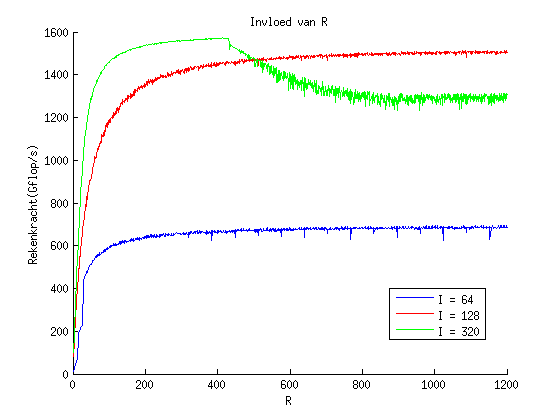
\includegraphics{invlR1200}
\caption{\label{invlR1200}Rekenkracht float16x16x16 voor verschillende waarden voor $R$ en $I$.}
\end{figure}

\begin{figure}
\centering
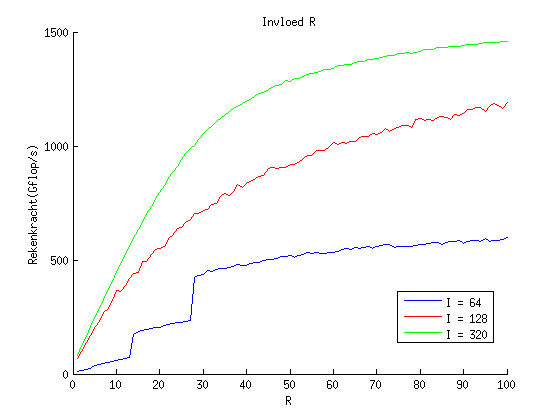
\includegraphics{invlR100}
\caption{\label{invlR100}Rekenkracht float16x16x16 voor verschillende waarden voor $R$ en $I$ met enkel de lage waardes van $R$.}
\end{figure}

\section{Invloed van I op kernels die $f(\T, \mUUU)$ berekenen}
\begin{figure}[h]
\centering
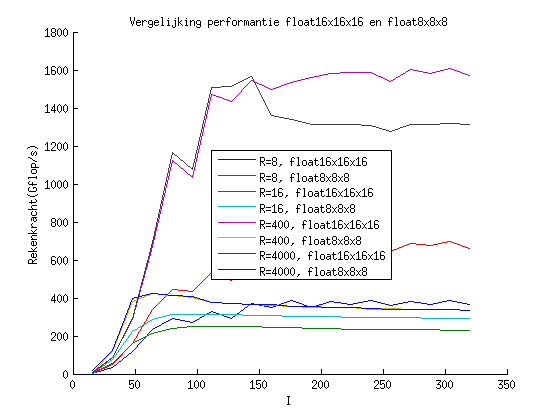
\includegraphics{fl16_vs_fl8_groot}
\caption{\label{fl16_vs_fl8} Vergelijking van de performantie tussen float16x16x16 en float8x8x8 voor verschillende waardes van $R$ en $I$.}
\end{figure}

We gebruiken in deze bespreking de kernels float16x16x16 en float8x8x8.
Voor elke kernel laten we $I$ oplopen van 16 tot en met 320 voor $R$ gelijk aan 8, 16, 400 en 4000. Zie figuur \ref{fl16_vs_fl8} voor de performantie van de kernels.

We laten $I$ oplopen in stappen van 16 omdat voor float16x16x16 $I$ een veelvoud moet zijn van 16. We beperken $I$ tot 320 omdat een buffer niet groter kan zijn dan 128MiB op onze grafische kaart. Als $I = 336$ dan moet de buffer om \TT{} op te slaan $336^3$ elementen $\times$ 4 B/element = 145MiB groot zijn.

We hebben voor $R$ de waardes 8 en 16 gekozen omdat dit twee punten zijn in de groeifase (zie figuur \ref{invlR100} en \ref{h:invlR}). $R=400$ is gekozen omdat het in de constante fase zit vlak voor dat rekenkracht terug naar beneden zakt. $R=4000$ is gekozen omdat het een hele grote waarde is die veel gewicht geeft aan de R-lus en dus heel performant moet zijn.

Bij $I$ = 16, 32 en 48 zien we een zeer sterke stijging van de performantie wanneer $I$ toeneemt. We kunnen die als volgt verklaren voor float16x16x16. Wanneer $I$ gelijk is aan 16 gebruiken we maar \'e\'en compute unit van de 24, wanneer $I$ gelijk is aan 32 gebruiken we er acht en bij 48 gebruiken we ze pas allemaal. Bij float8x8x8 gebruiken we voor $I=16$ acht CU's en vanaf $I=32$ alle CU's.

Nadat alle CU's in gebruik zijn zien we dat de rekenkracht nog steeds blijft stijgen. Dit komt omdat de CU's stil liggen wanneer alle work-groups op gegevens uit het globaal geheugen wacht. Door nog meer work-groups toe te wijzen aan een CU kunnen de CU's toch nog nuttige berekeningen doen terwijl andere work-groups op gegevens wachten. Dit verklaart waarom de rekenkracht toch sterk blijft stijgen nadat elke CU al minstens \'e\'en work-group uitvoert. Het is dus belangrijk om veel work-groups te voorzien.

Wanneer er genoeg work-groups zijn blijft de performantie min of meer constant. Bij float8x8x8 zien we amper schommelingen, terwijl we wel duidelijke schommelingen vaststellen bij float16x16x16. Merk wel op dat bij float16x16x16 de schommelingen gelijk lopen bij alle waardes van $R$.

Bij float16x16x16 met een $R=4000$ zien we dat bij $I=144$ de rekenkracht afneemt van 1566 Gflop/s naar ongeveer 1310 Gflop/s, net als bij \ref{h:invlR}. De verklaring is dezelfde als bij \ref{h:invlR}. Namelijk dat de caches niet zo goed meer werken.

Voor float16x16x16 zien we ook duidelijk dat de rekenkracht bijna lineair groeit met $R$ wanneer $R$ gelijk is aan 8 en 16. Wanneer $I$ groter is dan 150 is de rekenkracht bij $R=16$ bijna twee maal zo groot als bij $R=8$. Bij float8x8x8 is dat effect niet zo goed zichtbaar en is ook het verschil tussen $R=16$ en $R=400$ niet zo groot. Merk ook op dat bij float8x8x8 $R=400$ en $R=4000$ zo goed als volledig samenvallen.

De hoogste waard die we meten is 1610Gflop/s. Dit is bijna 60\% van de theoretisch maximale rekenkracht van de grafische kaart. We halen deze rekenkracht met float16x16x16 bij $R=400$ en $I=304$. De rest van de maximale rekenkracht gaat verloren naar het wisselen tussen work-groups op de compute-unit, redundante berekeningen, boekhoudkundige berekeningen zoals het berekenen van indexen en het niet volledig vullen van een VLIW.

\section{Vergelijking verschillende kernels die $f(\T, \mUUU)$ berekenen}
We hebben verschillende kernels ontwikkeld en willen die graag met elkaar vergelijken. Figuren \ref{fl16R_vs_fl16I}, \ref{fl16_vs_fl16R}, \ref{fl8_vs_fl8R} en \ref{fl16_vs_fl8} tonen de performantie van verschillende combinaties van de ontwikkelde kernels.

\subsection{Vergelijking tussen float16x16x16 en float16x16x16R}
\begin{figure}[h!]
\centering
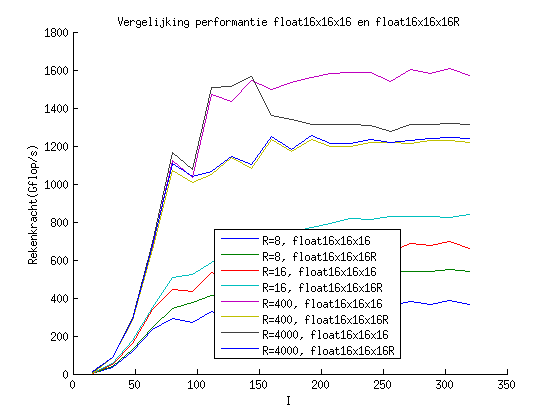
\includegraphics{fl16_vs_fl16R}
\caption{\label{fl16_vs_fl16R} Vergelijking van de performantie tussen float16x16x16 en float16x16x16R voor verschillende waardes van $R$ en $I$.}
\end{figure}

Float16x16x16R heeft als doel om het aantal geheugen conflicten te beperken. We willen graag zien of dit effectief gelukt is. Zie figuur \ref{fl16_vs_fl16R} voor een vergelijking van de performatie. We moeten een onderscheid maken tussen twee situaties. $R$ in de groeifase en $R$ in de constante fase.

Voor $R$ in de groeifase zien we dat float16x16x16R het duidelijk beter doet dan float16x16x16 wanneer $I$ wat groter is. Dit komt omdat in de groeifase de rekenkracht beperkt wordt door de bandbreedte. Door het aantal kanaalconflicten te verlagen kunnen we veel beter gebruik maken van die bandbreedte.

Wanneer $R$ in de constante fase is zijn de rollen omgekeerd. Na $I=96$ blijft de performantie van float16x16x16 verder groeien terwijl de performantie van float16x16x16R niet meer groeit.

Wanneer $I$ klein is zien we in alle gevallen dat float16x16x16 en float16x16x16R nagenoeg samenvallen. Dit komt omdat de kanaalconflicten dan nog niet het knelpunt is en dus slechts een beperkte, maar wel zichtbare, invloed hebben op de performantie.



\subsection{Vergelijking tussen float16x16x16R en float16x16x16I}
\begin{figure}[h!]
\centering
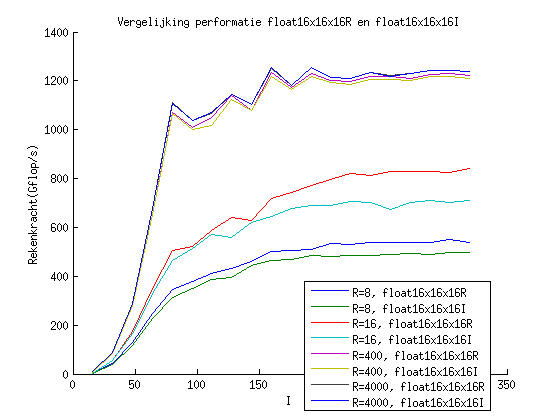
\includegraphics{fl16R_vs_fl16I}
\caption{\label{fl16R_vs_fl16I} Vergelijking van de performantie tussen float16x16x16R en float16x16x16I voor verschillende waardes van $R$ en $I$.}
\end{figure}

Float16x16x16R en float16x16x16I zijn beiden kernels die als doel hebben om het aantal geheugen conflicten te beperken. Zie figuur \ref{fl16R_vs_fl16I} voor een vergelijking van de performatie. We zien duidelijk dat float16x16x16R het overal beter doet dan float16x16x16I. Daarom gaan we verder geen aandacht meer besteden aan float16x16x16I.

\subsection{Vergelijking tussen float16x16x16 en float8x8x8}

\begin{figure}[h!]
\centering
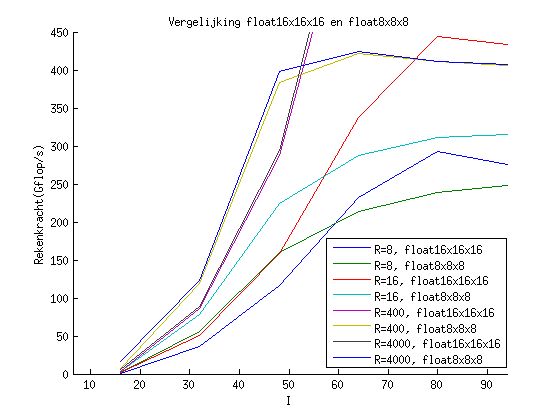
\includegraphics{fl16_vs_fl8_klein}
\caption{\label{fl16_vs_fl8_klein} Vergelijking van de performantie tussen float16x16x16 en float8x8x8 voor verschillende waardes van $R$ en $I$, uitvergroting snijpunten.}
\end{figure}

Zie figuur \ref{fl16_vs_fl8} voor een vergelijking tussen float16x16x16 en float8x8x8. Voor $I$ groter dan 64 zien we dat float16x16x16 veel beter presteert dan float8x8x8. Dit komt omdat float16x16x16 veel minder redundante berekeningen en geheugenoperaties moet doen dan float8x8x8. (Zie \ref{h:fl8_rekenverhouding} onder het punt 'Rekenverhouding')

Maar float8x8x8 heeft ook een voordelen. Omdat een work-group maar 8$\times$8$\times$8 groot is, zijn er meer work-groups nodig voor dezelfde hoeveelheid elementen. Waardoor de CU's beter benut worden. Zie figuur \ref{fl16_vs_fl8_klein} voor een beter zicht hierop. We zien dat float8x8x8 beter presteert dan float16x16x16 wanneer $I$ nog klein is. Het is pas later dat float16x16x16 de bovenhand haalt.

\subsection{Vergelijking tussen float8x8x8 en float8x8x8R}

\begin{figure}[h!]
\centering
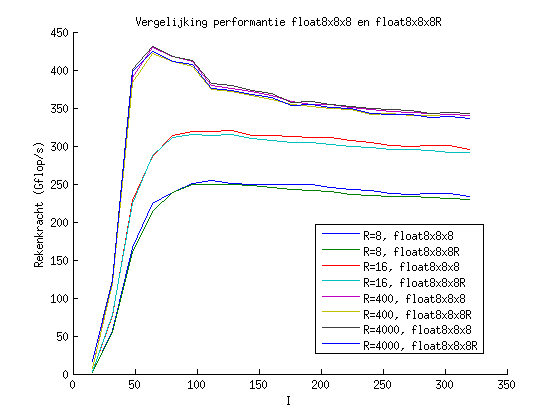
\includegraphics{fl8_vs_fl8R}
\caption{\label{fl8_vs_fl8R} Vergelijking van de performantie tussen float8x8x8 en float8x8x8R voor verschillende waardes van $R$ en $I$.}
\end{figure}

Zie figuur \ref{fl8_vs_fl8R} voor een vergelijking tussen float8x8x8 en float8x8x8R. We zien dat float8x8x8 het er overal een heel klein beetje beter doet dan float8x8x8R. We kunnen dus beter geen aandacht besteden aan float8x8x8R.

\section{Kernels die \GGG{} berekenen}
\begin{figure}[h!]
\centering
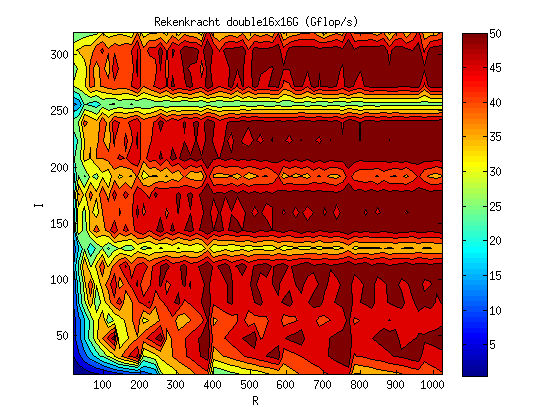
\includegraphics{result_gradient}
\caption{\label{result_gradient} Rekenkracht double16x16G in functie van $R$ en $I$}
\end{figure}

Zie figuur \ref{result_gradient} voor de rekenkracht van double16x16G in functie van $R$ en $I$. We hebben $I$ laten oplopen van 16 tot en met 320 in stappen van 16, en $R$ van 16 tot en met 1024 in stappen van 16.

Wat meteen opvalt is dat de performantie sterk daalt wanneer $I$ een veelvoud is van 64. We kunnen dit niet verklaren maar we vermoeden dat het veroorzaakt kan worden door de ligging van de elementen in het geheugen.

Wanneer we naar de waardes van de rekenkracht kijken zien we dat we niet meer dan 54 Gflop/s halen in dubbele precisie. Dit is amper 8\% van de capaciteit van de grafische kaart.

\section{Besluit}

De kernels die $f(\T, \mUUU)$ berekenen doen het heel goed met zelfs waardes van 1610 Gflop/s. Dat is bijna 60\% van de capaciteit van de grafische kaart. 

Float8x8x8 doet het beter dan float16x16x16 bij lage waardes van $I$ omdat er meer work-groups zijn en float16x16x16R doet het beter dan float16x16x16 wanneer $R$ laag is omdat die effi\"enter om gaat met het globaal geheugen. Deze drie kernels vullen elkaar dus goed aan. Float16x16x16I en float8x8x8R doen hun werk vrij goed, maar in elke situatie is er wel een andere kernel die net iets performanter is.

De kernel om \GGG{} te berekenen haalt slechts 8\% van de capaciteit van de grafische kaart en doet het dus niet goed.
% ... en zo verder tot
\chapter{Besluit}
\label{besluit}
De masterproeftekst wordt afgesloten met een hoofdstuk waarin alle
besluiten nog eens samengevat worden. Dit is ook de plaats voor suggesties
naar het verder gebruik van de resultaten, zowel industri"ele toepassingen
als verder onderzoek.

\lipsum[1-7]

%%% Local Variables: 
%%% mode: latex
%%% TeX-master: "masterproef"
%%% End: 


% Indien er bijlagen zijn:
\appendixpage*          % indien gewenst
\appendix
\chapter{Broncodes kernels}
%\section{Kernels om $f(\T, \mUUU)$ te berekenen}
\label{app:A}
In deze appendix kan u de volledige broncodes vinden voor alle besproken kernels uit hoofdstuk \ref{h:kernels}. Ze staan in de volgorde waarin ze besproken worden in de tekst. We raden de lezer aan om de broncodes stap voor stap te bestuderen. Zo zal de lezer sneller inzicht krijgen in de structuur van de geavanceerde kernels. Omdat niet alle kernels op \'e\'en blad passen gaan we de ondertitels boven de code zetten.

\newpage
\lstinputlisting[caption={Broncode van de eerste kernel.}, label={codeFloat}]{opencl/float.cl}

\newpage
\lstinputlisting[caption={Broncode van de eerste kernel met 64 work-items.}, label={codeFloat64}]{opencl/float64.cl}

\newpage
\lstinputlisting[caption={Broncode van float4x4x4.}, label={codeFloat4x4x4}]{opencl/float4x4x4.cl}

\newpage
\lstinputlisting[caption={Broncode van float8x8x8.}, label={codeFloat8x8x8}]{opencl/float8x8x8.cl}

\newpage
\lstinputlisting[caption={Broncode van float16x16x16.}, label={codeFloat16x16x16}]{opencl/float16x16x16.cl}

\newpage
\lstCode{float8x8x8R}

\newpage
\lstCode{float16x16x16R}

\newpage
\lstCode{float8x8x8Mapper}

\newpage
\lstCode{float16x16x16Mapper}

\newpage
\lstCode{float16x16x16I}

\newpage
\lstCode{float16x16x16MapperI}

\newpage
\lstCode{double16x16x16FG}
%%% Local Variables: 
%%% mode: latex
%%% TeX-master: "masterproef"
%%% End: 

% ... en zo verder tot
\chapter{De laatste bijlage}
\label{app:n}
In de bijlagen vindt men de data terug die nuttig kunnen zijn voor de
lezer, maar die niet essentieel zijn om het betoog in de normale tekst te
kunnen volgen. Voorbeelden hiervan zijn bronbestanden,
configuratie-informatie, langdradige wiskundige afleidingen, enz.

\section{Lorem 20-24}
\lipsum[20-24]

\section{Lorem 25-27}
\lipsum[25-27]

%%% Local Variables: 
%%% mode: latex
%%% TeX-master: "masterproef"
%%% End: 


\backmatter
% Na de bijlagen plaatst men nog de bibliografie.
% Je kan de  standaard "abbrv" bibliografiestijl vervangen door een andere.
\bibliographystyle{abbrv}
\bibliography{referenties}

\end{document}

%%% Local Variables: 
%%% mode: latex
%%% TeX-master: t
%%% End: 
